
The motivation for each of the detector uncertainty is detailed here.
There are three ways of implementing the \Gls{ND} detector systematic
uncertainties in \Gls{TK}, the first ones are called ``variation
systematics'', where the physical quantity (momentum and \Gls{TPC}
\Gls{PID} pull) that is being measured is changed according to the
effect of the systematic; another type controls the normalisation of a
whole class of events (so-called ``normalisation-like systematics'')
and finally, ``efficiency-like systematics'' which control, on an
event by event basis the weight of an event. All the uncertainties
that comes from detector effects are described here.

\subsection{Variation systematic uncertainties}

\subsubsection{The momentum scale uncertainty}
\label{subsec:momscale}
The magnetic field has an absolute error of $0.57\%$ that gets
directly propagated on the momentum of the particle~\cite{TN212}.

\subsubsection{The magnetic~/~electric field uncertainty}
\label{subsubsec:bfield}
The magnetic and electric field uncertainty~\cite{TN212} comes from
the fact that both the fields are not uniform in the \Gls{TPC}. This
is due to the presence of various equipment around the \Gls{TPC} or
the \Gls{TPC} case itself which produce fringe fields. In general, the
magnetic field and these fringe fields make the drift electrons from
the ionisation travel in a line which is not straight, which makes the
reconstruction more complicated. Some corrections can be applied at
the reconstruction level to take this effect into account, but there
is still a systematic uncertainty which has applied to the
reconstructed momentum.

On the cathode, some ``dots'' can be illuminated by lasers to produce
photo-electrons. These electrons drift until the readout plane, and
one can estimate the error on the corrections by calculating distance
from the reconstructed position of the dots to their real position.
This leads, at the analysis level, to an uncertainty on the momentum
of the particle.

\subsubsection{The momentum resolution uncertainty}
\label{subsec:momresol}
The \Gls{TPC} momentum resolution~\cite{TN212} was computed with
through going tracks that are reconstructed in multiple
\Glspl{TPC}. This systematic uncertainty aims at characterising the
intrinsic momentum resolution of the \Glspl{TPC}. The presence of
intermediate \Glspl{FGD} complicates the error calculation, as one
needs to correct for momentum loss in them. The uncertainty is
propagated on $1 / p_T$ where $p_T$ is the transverse momentum of the
particle (where transverse means orthogonal to the $Z$ direction, in
the $ZY$ plane). The uncertainty is around $10^{-4}$ for a
$500\text{~MeV}$ particle. This uncertainty is directly propagated on
the momentum of the particle.

\subsubsection{The \Gls{TPC} \Gls{PID} uncertainty}
\label{subsec:tpcpid}
The \Gls{PID} quantities that are used are the pulls, defined from the
$dEdx$ as shown in Equation~(\ref{eq:tpcpull}). To get an uncertainty
on these quantities, the pull is calculated for control samples on a
subset of the data available. This is then compared to the expected
\Gls{MC} distribution. In this case, the control sample is a photon
sample (electron~/~positron pairs with an invariant mass and good
\Gls{TPC} quality requirements). One obtains distributions similar to
the one shown in Figure~\ref{fig:tpcsyst} and can compare the width
and position of the Gaussian distributions which are used as
systematic uncertainties. In Figure~\ref{fig:tpcsyst}, on the right,
each of the data and \Gls{MC} distributions (in blue and green
histograms, respectively) are fitted with Gaussian functions (blue and
green curves). The \Gls{MC} predictions are then shifted to overlap
with the data by moving the mean of the Gaussian function for \Gls{MC}
and its spread, thus producing a correction that has to be applied to
the nominal \Gls{MC}.

The systematic uncertainty comes from the errors on the parameters of
the Gaussian functions, which is retrieved from the fit.

This is repeated for different momentum bin, particle type and, if the
statistics are sufficient, run period and \Gls{TPC} (in practice, this
split can only be realised for muons)~\cite{TN212}.

\begin{figure}[ht]
  \center
  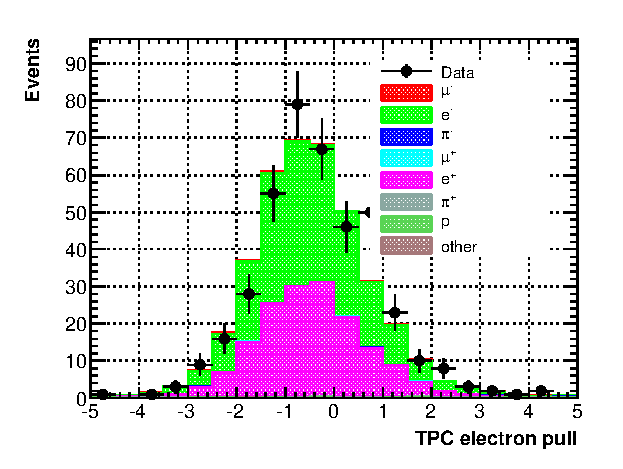
\includegraphics[width=0.48\textwidth]{T2K-TN-254/images/corrections/nopidcor_lowMom.eps}
  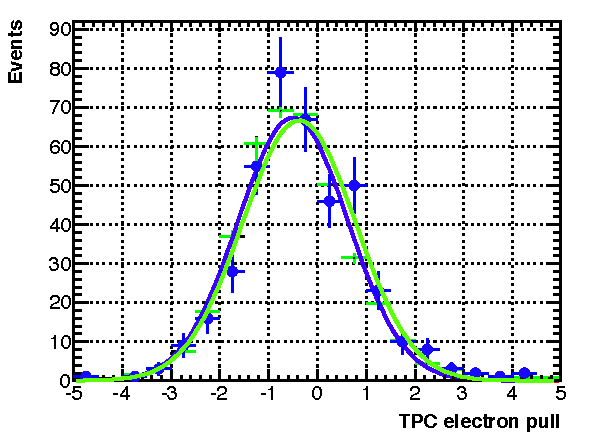
\includegraphics[width=0.48\textwidth]{T2K-TN-254/images/corrections/pidcorr_lowMom_fit.pdf}
  \caption[PID pull for electrons (or positrons) of momentum smaller
  than $200$~MeV]{\textbf{\textit{Left:}} \Gls{PID} pull for electrons
    (or positrons) of momentum smaller than $200$~MeV.
    \textbf{\textit{Right:}} \Gls{PID} pull Gaussian fits for data
    (blue) and \Gls{MC} (green).}
  \label{fig:tpcsyst}
\end{figure}


\subsection{Efficiency systematic uncertainties}
The efficiency systematic errors are applied to the events and in
general are applied to both the pair and main tracks, unless stated
otherwise.

\subsubsection{The \Gls{TPC} cluster efficiency uncertainty}
\label{subsec:tpccluster}
The \Gls{TPC} cluster efficiency uncertainty~\cite{TN212} is applied
because there is a cut on the number of nodes the tracks creates in
the \Gls{TPC} (track quality cut). Note that clusters are horizontal
or vertical hits that are joined together (see the step~2 in the
\Gls{TPC} paragraph in Section~\ref{subsubsec:reconstruction}). This
was computed by comparing the number of nodes of muon data control
samples to its equivalent in the \Gls{MC}. These control samples are a
subset of a \Gls{CC} inclusive selection and cosmic muons
triggers. The selections are run without the \Gls{TPC} track quality
and the ratios
\begin{align}
  &\frac{\epsilon_\text{Data}}{\epsilon_\text{MC}} \label{eq:effcorrection}\\
  &\text{and~}\frac{\epsilon_{\text{MC}}-\epsilon_{\text{Data}}}{\epsilon_{\text{MC}}}\label{eq:efferror}
\end{align}
are computed (in these equations, $\epsilon$ indicate the data and
\Gls{MC} efficiency). It was then found that shifts one has to apply
to the \Gls{MC} (first ratio) and error (second ratio) are both the
order of one per mil.

\subsubsection{The \Gls{TPC} track efficiency uncertainty}
\label{subsubsec:tpctrack}
The \Gls{TPC} track efficiency uncertainty~\cite{TN212} characterises
the error one gets by solely requiring the presence of a track in the
\Gls{TPC}. Rather than cluster efficiency, this error is related to
the presence of a full reconstructed object as explained in the
\Gls{TPC} paragraph of Section~\ref{subsubsec:reconstruction} (step
3). The error is computed with through-going muons which cross several
detectors. The data and \Gls{MC} comparison for such sample show that
there is no unexpected behaviour in the all \Glspl{TPC} and that the
uncertainty does not depend on the momentum, position and number of
track crossing them. The error is around $0.5\%$ for a single track
entering the \Gls{TPC}2.

\subsubsection{The \Gls{TPC}~/~\Gls{FGD} matching efficiency uncertainty}
\label{subsubsec:tpcfgdmatch}
The \Gls{TPC}~/~\Gls{FGD} matching efficiency uncertainty~\cite{TN212}
arises because the tracks in the selection have to be reconstructed as
a single object. Note that, even though there is no explicit
requirement for the Pair Track to be in the \Gls{FGD} (only a distance
specification is made), there is a priori, no requirement to apply
this error for cases where the Pair Track does not use the
\Gls{FGD}. However this was considered to be a marginal effect that
happens only if the Main Track is next to the \Gls{TPC}, on the edge
of the \Gls{FGD}, so it was applied regardless of the topology of the
Pair Track.

The efficiency was computed using through-going muons crossing
different \Glspl{TPC}, and found to be exactly $100\%$ (i.e. no track
that enter the \Gls{TPC} from the \Gls{FGD} are missed, and vice
versa). Recalling that the \Gls{FGD}1 \Gls{FV} extends to the last
layer downstream, right next to the \Gls{TPC}2, and that only two bars
are removed in the upstream direction, this is maybe not
surprising. To assign the error, it was decided that the \Gls{TPC} /
\Gls{FGD} matching could fail if a track leaves only two hits in the
\Gls{FGD} (i.e. it is very close to its edge) and therefore the hit
efficiency is used as the error, which in this case is equal to about
$0.8\%$.

\subsubsection{The \Gls{TPC}~/~\Gls{ECal} matching efficiency uncertainty}
\label{subsubsec:tpcecalmatch}
It was found recently that the \Gls{ECal}'s representation in the
\Gls{MC} was few millimetres away from its real position. Therefore
there could be a mismatch between the probability in reconstructing a
particle in the \Gls{ECal} which came from the \Gls{TPC} in data and
\Gls{MC}. This could affect the \Gls{ECal} veto since there is a
requirement for the selected veto object to not be one of the two
tracks. An uncertainty is therefore applied on the \Gls{MT} of
\Gls{PT} when they enter the \Gls{ECal}. The uncertainty which is
propagated on these tracks is of the order of $5\%$~\cite{TN279}.

\subsubsection{Charge Identification uncertainty}
\label{subsubsec:chargeid}
The charge identification is a fundamental input to the analysis,
since it relies on the selection of two tracks of opposite charge.
The error that is used is determined from the control samples which
have a muon traversing several \Glspl{TPC}~\cite{TN212}. One can then
compare the probability to incorrectly swap the charge between data
and \Gls{MC}. The error decreases with the number of \Gls{TPC} the
particle traverses; in the worst case, when the track is reconstructed
in two \Glspl{TPC}, and each one reconstructs a different charge, the
uncertainty is of $2\%$.  The error is propagated on the inverse
transverse momentum as in the case of the momentum resolution.

\subsection{Normalisation uncertainties}
These uncertainties are applied to a whole class of events based on
their topologies, it generally does not rely on the detector
efficiencies themselves, but rather on other effects such as the cross
section (for the pion and proton secondary interaction), the mass
uncertainties (for the photon secondary interactions and the \Gls{FGD}
mass), or the presence of additional events (pile up uncertainties).

\subsubsection{\Gls{FGD} mass uncertainty}
\label{subsec:fgdmass}
The \Gls{FGD} has a mass uncertainty of $0.6\%$, which comes from the
uncertainty in size of its bars and the hole for the
fibre~\cite{TN212}.

\subsubsection{The pile up and sand uncertainties}
\label{subsec:pileup}
The pile up uncertainty comes from the fact that vetoes are present in
the selection. Indeed, additional ``\gls{sand}'' events that comes
from the sand around the \Gls{ND} can reach the detector and trigger
the veto of the selection. In the interest of time and space, these
events are not included in the standard ``\gls{magnet} \Gls{MC}''
(i.e. events that are in happening the volume enclosed by the \Gls{ND}
magnet) that is used for the analysis, they are added separately. The
problem is then, since these ``\gls{sand}'' events are added
separately on top of the simulation, how to see their effect on the
vetoes? For example, if a ``\gls{magnet}'' event is selected and
passes the selection, and if there was a ``\gls{sand}'' in the same
time, one would expect to select fewer events. Hence the name, the
magnet and sand events are ``piled up.''

The way to overcome this is by calculating a pile up correction and
uncertainty. For that, the strategy is to run a selection which only
has the vetoes, and comparing the data to the sum of the \gls{magnet}
\Gls{MC} and \gls{sand} \Gls{MC}. The vetoes are added in the same
order as in the selection.

Note that the \gls{sand} events have an intrinsic uncertainty of
$10\%$, which comes from the simulation of the surroundings of the
\Gls{ND}, the flux uncertainty and the cross section.

Upon assigning the pile up correction, the strategy is to modify the
normalisation of the whole selection based on the \gls{sand} trigger
rate one gets. The error is either the data~/~\Gls{MC} difference, or
the \gls{sand} error if it is greater than the former. All the errors
and corrections are listed in Table~\ref{tab:pileup}, note that the
correction is dependent on the run, since the \Gls{MR} power increases
and produces different yields in the vetoes due to the expected
increase in \gls{sand} interaction and thus pile up.

\begin{table}[ht]
  \center
  \begin{tabular}{cccc}
    \toprule
    Veto & Run & Correction & Systematic uncertainty \\
    \cmidrule(r){1-4}
    \multirow{6}{*}{\Gls{TPC} muon rejection} & 2A  & 0.992 & 0.009 \\
         & 2W  & 0.993 & 0.007 \\
         & 3AB & 0.994 & 0.009 \\
         & 3AC & 0.991 & 0.009 \\
         & 4A  & 0.989 & 0.010 \\
         & 4W  & 0.990 & 0.010 \\
    \cmidrule(r){1-4}                        
    \multirow{6}{*}{\Gls{TPC} Veto} & 2A  & 0.995 & 0.008 \\
         & 2W  & 0.996 & 0.007 \\
         & 3AB & 0.996 & 0.008 \\
         & 3AC & 0.994 & 0.009 \\
         & 4A  & 0.992 & 0.010 \\
         & 4W  & 0.994 & 0.010 \\
    \cmidrule(r){1-4}                        
    \multirow{6}{*}{\Gls{PD} Veto} & 2A  & 0.928 & 0.009 \\
         & 2W  & 0.936 & 0.008 \\
         & 3AB & 0.937 & 0.009 \\
         & 3AC & 0.920 & 0.010 \\
         & 4A  & 0.897 & 0.012 \\
         & 4W  & 0.906 & 0.010 \\
    \cmidrule(r){1-4}
    \multirow{6}{*}{\Gls{ECal} Veto} & 2A  & 0.9989 & 0.0006 \\
         & 2W  & 0.9983 & 0.0007 \\
         & 3AB & 0.9991 & 0.0007 \\
         & 3AC & 0.9979 & 0.0008 \\
         & 4A  & 0.9974 & 0.0008 \\
         & 4W  & 0.9967 & 0.0010 \\

    \bottomrule
  \end{tabular}
  \caption[Pile up corrections and systematic uncertainties used in
  the analysis]{Pile up corrections and systematic uncertainties used
    in the analysis.}
  \label{tab:pileup}
\end{table}

Finally, as no \gls{sand} event enters the actual selection, they thus
lead to no additional uncertainty.

\subsubsection{The pion secondary interaction uncertainty}
\label{subsec:pionsec}
The pion secondary interaction uncertainty~\cite{TN212} is a weight
error that is propagated on the events which have charged pions in
them. A secondary interaction happens when this pion reinteracts with
some of the detector material, rather than losing energy by ionisation
in the detector.

There are a lot of channels in which a charged pion can interact, but
the most important in the context of this analysis is the charge
exchange channel, where a pion goes from being a charged pion to a
neutral pion after interaction with a nucleus. Unfortunately, the
\Gls{MC} model that was implemented in the \Gls{ND} simulations
(Bertini model~\cite{WRIGHT2015175}) was found to very poorly describe
the available data at \Gls{TK}
energies~\cite{TN125,TN325,Ashery:1981tq} ($200\text{~MeV}$);
therefore a correction factor was included in the cross section for
charged pions. The error on the above mentioned
data~\cite{Ashery:1981tq} was also propagated to the weight to be able
to get an uncertainty on the secondary pion interaction. Note that
these are completely uncorrelated with the \Gls{FSI} errors as
described earlier; correlating the pion secondary interaction and the
\Gls{FSI} will constitute an improvement for the next generation of
analyses at the \Gls{ND}.

\subsubsection{The proton secondary interaction uncertainty}
\label{subsec:protonsec}
The proton secondary interaction probability uncertainty~\cite{TN212}
is propagated if the \Gls{MT} or \Gls{PT} is a proton. This happens if
the \Gls{PID} did not work properly, for example. The low energy
protons have a probability of interacting with the scintillator in the
\Gls{FGD} and can reinteract in it. A very conservative error of
$10\%$ is applied for the proton interactions.

\subsubsection{The photon secondary interaction uncertainty}
\label{subsec:photonsec}
\input{T2K-TN-313/systematicsoofv.tex}

\subsubsection{Out of fiducial volume reconstruction uncertainty}
\label{subsec:recooofv}
This uncertainty is propagated because the \Gls{MT} and \Gls{PT} are
selected inside the \Gls{FV} of the detector. This was based on work
from~\cite{TN098}. It can happen that the tracks come from outside the
fiducial volume but are reconstructed inside if for example there was
a failure to detect a hit in the outer layers of the \Gls{FGD}, or a
hard scatter in the \Gls{FGD} that somehow confuses the
reconstruction. These can sometime have a large uncertainty ($30$ to
$50\%$) depending on the topology of the track.


\subsection{Summary of the detector uncertainties}
\label{subsec:detsystsummary}

Table~\ref{tab:detectoruncertaintyinfv} gives a summary of the overall
effects of all the detector errors. Note that in this table, the
positive and negative errors are determined using the \Gls{HPD}
(Highest Posterior Density) method\footnote{The following method was
  used to calculate the error of a distribution:
  \begin{itemize}[noitemsep,topsep=0pt]
  \item Find the mode of the distribution, which is now referred as
    $N_\text{event}^\text{mode}$,
  \item Create an interval for which the \Gls{PDF} is constant and
    contain the $68\%$ of the total distribution,
  \item Read off the values corresponding to the number of events (on
    the X axis) the positive and negative values are called
    $N_\text{event}^{\pm}$,
  \item Use the values
    $\frac{\left|N_\text{event}^\text{mode} -
        N_\text{event}^\pm\right|}{N_\text{event}^\text{mode}}$ as the
    positive and negative relative uncertainties. \label{ftn:hpd}
  \end{itemize}
}. Note that this method is quite sensitive to the number of toy
thrown and the binning chosen for the computation.

Figure~\ref{fig:detectorsystematicsinfv} shows the \Gls{PDF} of the
selected event after propagation of the detector errors.

\begin{table}[ht]
  \center
  \begin{tabular}{ll}
    \toprule
    Systematic & Relative uncertainty \\
    \midrule
    \multicolumn{2}{l}{Weight errors} \\
    \midrule
    Charge identification efficiency         & 0.002  \\
    \Gls{TPC} cluster efficiency             & 0.000009\\
    \Gls{TPC} track efficiency               & 0.011  \\
    \Gls{TPC}~/~\Gls{FGD} matching efficiency& 0.006  \\
    \Gls{TPC}~/~\Gls{ECal} matching efficiency & $< 0.00001$  \\
    \Gls{FGD} mass                           & 0.043  \\
    Secondary interaction pion               & 0.046  \\
    Secondary interaction proton             & 0.026  \\
    Secondary interaction photon             & $\pm^{0.41}_{0.15}$  \\
    Reconstructed \Gls{OOFV}                 & 0.061  \\
    \Gls{ECal} pile up                       & 0.0004 \\
    Muon rejection pile up                   & 0.0004  \\
    \Gls{PD} pile up                         & 0.006  \\
    \Gls{TPC} pile up                        & 0.005  \\
    \midrule
    \multicolumn{2}{l}{Variation errors} \\
    \midrule
    Magnetic field      & 0.009 \\
    Momentum scale      & 0.022 \\
    Momentum resolution & 0.025 \\
    \Gls{TPC} \Gls{PID} & 0.019 \\
    \midrule
    Total & $\pm^{1.24}_{0.20}$ \\
    \bottomrule
  \end{tabular}
  \caption[Detector uncertainties for the selected events]{Relative
    detector uncertainties for the events that pass the selection.}
  \label{tab:detectoruncertaintyinfv}
\end{table}

\begin{figure}[ht]
  \center
  \includegraphics[width=0.8\textwidth]{images/NCg/Det.pdf} 
  \caption[Effect of the detector uncertainty on the number of
  selected events]{Effect of the detector uncertainty on the number of
    selected events. The nominal central value is indicated by the
    arrow.}
  \label{fig:detectorsystematicsinfv}
\end{figure}


%%% Local Variables:
%%% mode: latex
%%% TeX-master: "Thesis"
%%% End:
